\documentclass[12pt,a4paper]{report}

% ── Core packages ──────────────────────────────────────────
\usepackage[a4paper, margin=2.5cm]{geometry}
\usepackage{graphicx}
\graphicspath{{images/}}
\usepackage{booktabs}
\usepackage{array}
\usepackage{longtable}
\usepackage{float}
\usepackage{caption}
\usepackage{xcolor}
\usepackage{hyperref}
\usepackage{parskip}
\usepackage{setspace}
\usepackage{enumitem}
\usepackage{pifont}   % for \checkmark via \ding{51}
\usepackage{amssymb}  % for \checkmark

\onehalfspacing

\hypersetup{
    colorlinks=true,
    linkcolor=black,
    urlcolor=blue,
    citecolor=black
}

% ── Title info ─────────────────────────────────────────────
\title{
    \textbf{AgriSmart} \\[0.5em]
    \large Intelligent Fertilizer and Pesticide Sprinkling System \\[0.5em]
    \normalsize Sprint Planning and Execution Methodology \\[1em]
    \normalsize 21CSP302L — Minor Project \\
    \normalsize SRM Institute of Science and Technology
}
\author{
    Sanchai K B \quad [RA2311026010342] \\
    Gokul Uday \quad [RA2311026010402]
}
\date{April 2026}

% ──────────────────────────────────────────────────────────
\begin{document}
% ──────────────────────────────────────────────────────────

\maketitle
\tableofcontents
\newpage

% ============================================================
\chapter{Sprint Planning and Execution Methodology}
% ============================================================

This chapter documents the Agile sprint methodology adopted for the development of AgriSmart. The project was structured into three two-week sprints, each with clearly defined goals, user stories, functional deliverables, architectural decisions, UI designs, functional test cases, daily progress logs, velocity tracking, and retrospective reviews.

\begin{figure}[H]
    \centering
    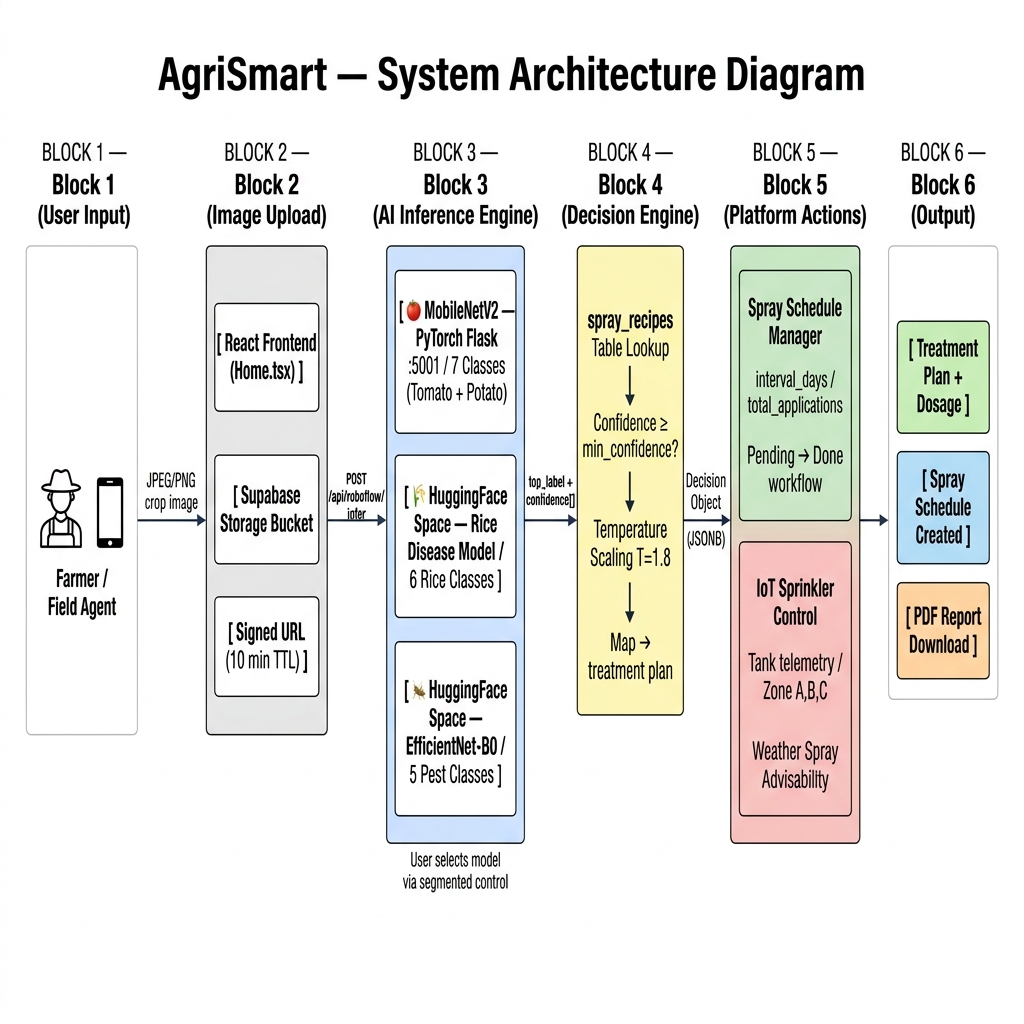
\includegraphics[width=\textwidth]{system_arch.png}
    \caption{AgriSmart --- Overall System Architecture (Component \& Deployment View)}
    \label{fig:system_arch}
\end{figure}

The overall system, shown in Figure~\ref{fig:system_arch}, follows a six-block data flow from user input through image upload, AI inference, decision engine processing, platform action management, and final output delivery.

% ============================================================
\section{Sprint 1 --- Foundation and Core AI Pipeline}
% ============================================================

\subsection{Sprint Goal with User Stories}

\textbf{Sprint Goal:} Establish the project's technical foundation and deliver a functional end-to-end AI inference pipeline that allows a farmer to upload a crop image and receive a disease or pest classification with an actionable spray recommendation.

\medskip
\textbf{Sprint Duration:} 2 Weeks \hfill \textbf{Sprint Number:} 1 of 3

\begin{table}[H]
\centering
\caption{Sprint 1 --- User Stories}
\label{tab:sprint1_us}
\renewcommand{\arraystretch}{1.4}
\begin{tabular}{|p{1.4cm}|p{7.8cm}|p{2.4cm}|p{1.8cm}|}
\hline
\textbf{ID} & \textbf{User Story} & \textbf{Priority} & \textbf{Status} \\
\hline
\#US01 & As a farmer, I want to upload a plant image through the web app so that I can check if my crop is healthy or diseased. & Must Have & Done \\
\hline
\#US02 & As a farmer, I want to see the spray recommendation clearly on my screen so that I know exactly what fertilizer or pesticide to apply. & Must Have & Done \\
\hline
\#US03 & As a farmer, I want a warning when the AI is not confident so that I know when to retake the photo. & Must Have & Done \\
\hline
\#US04 & As a farmer, I want the application to work on my mobile phone so that I can use it directly in the field. & Must Have & Done \\
\hline
\end{tabular}
\end{table}

\subsection{Functional Document}

The primary functional deliverable of Sprint 1 was the construction and training of two deep learning models --- one for insect/pest classification and one for rice disease classification --- along with the Flask-based inference server that serves predictions in response to image uploads from the React frontend.

The \textbf{insect classifier} is based on the ResNet18 architecture, loaded with ImageNet-pretrained weights (\texttt{IMAGENET1K\_V1}). The model's fully connected head was replaced with a custom Sequential block comprising a Dropout layer (rate: 0.4) followed by a Linear layer mapping from ResNet18's 512-dimensional feature space to five target pest classes. All backbone parameters were frozen and only the final residual block (\texttt{layer4}) was unfrozen for gradient updates. The best validation accuracy recorded was \textbf{87.24\%}.

The \textbf{rice disease classification model} employs EfficientNet-B0, also initialized with ImageNet weights. All layers were unfrozen during fine-tuning. The classifier head was replaced with Dropout(0.5) and a Linear layer projecting to six rice disease classes. Best validation accuracy: \textbf{86.06\%}.

Both models are served through a unified Flask inference server (port 5001). Images are preprocessed: resized to $224 \times 224$\,px, normalized with ImageNet statistics (mean: [0.485, 0.456, 0.406], std: [0.229, 0.224, 0.225]), converted to a PyTorch tensor, and passed through the model inside a \texttt{torch.no\_grad()} context. Softmax probabilities are returned as JSON.

\subsection{Architecture Document}

Sprint 1 established a clean three-tier architecture:

\begin{itemize}
    \item \textbf{Client Tier:} React application with image upload (drag \& drop), model selector toggle (Pest / Disease), and Analysis Report output panel.
    \item \textbf{Server Tier:} Flask inference server (:5001) with two model checkpoints loaded in memory. POST requests routed by model type.
    \item \textbf{Data Tier:} Supabase PostgreSQL (\texttt{diagnoses} table) and Supabase Storage (\texttt{diagnosis-images} bucket) with Row Level Security (RLS).
\end{itemize}

\begin{figure}[H]
    \centering
    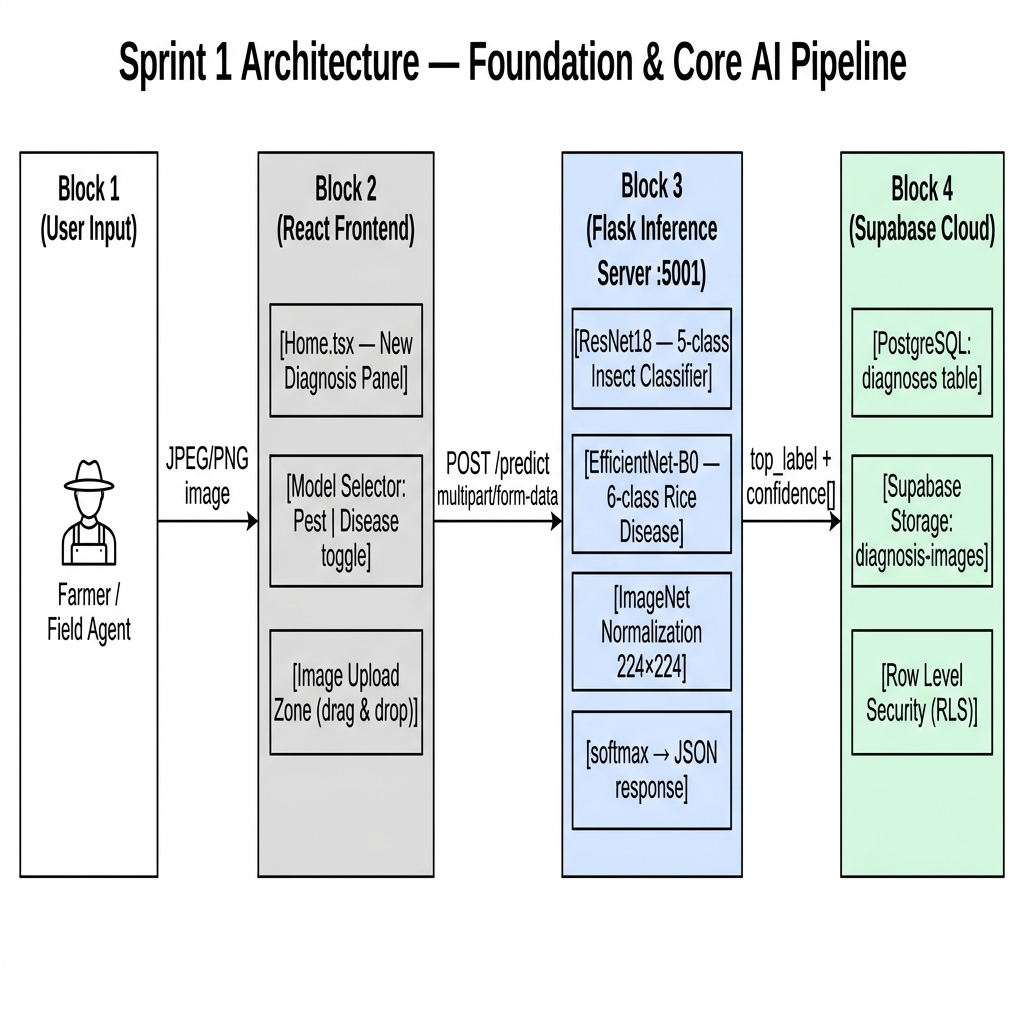
\includegraphics[width=\textwidth]{sprint1_arch.png}
    \caption{Sprint 1 Architecture --- Foundation \& Core AI Pipeline}
    \label{fig:sprint1_arch}
\end{figure}

As illustrated in Figure~\ref{fig:sprint1_arch}, the user submits a JPEG/PNG image through the React frontend which dispatches a \texttt{multipart/form-data} POST request to the Flask inference server. The server processes the image through the CNN pipeline and returns a ranked class prediction with confidence scores. The result is persisted to Supabase and rendered in the Analysis Report panel.

\subsection{UI Design}

The Dashboard presents a clean, two-panel layout. The left panel (\textit{New Diagnosis}) contains the model selector, a drag-and-drop image upload zone, and an \textit{Analyze Image} button. The right panel (\textit{Analysis Report}) renders the Detected Condition label, an \textbf{Action Required} or \textbf{Healthy} status badge, a confidence score progress bar, the AI Recommendation, and special field notes.

\begin{figure}[H]
    \centering
    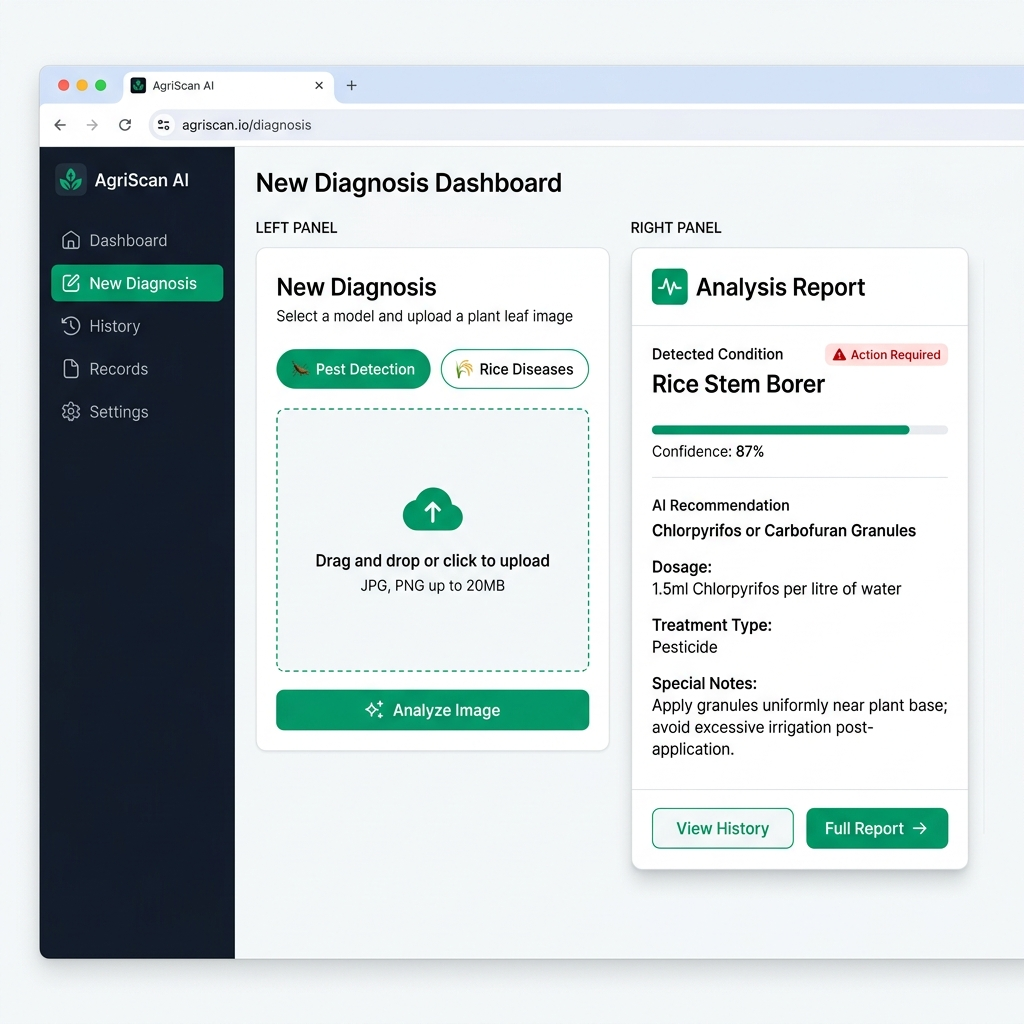
\includegraphics[width=\textwidth]{sprint1_ui.png}
    \caption{Sprint 1 UI --- New Diagnosis Dashboard with Analysis Report Panel}
    \label{fig:sprint1_ui}
\end{figure}

Figure~\ref{fig:sprint1_ui} shows the Sprint 1 dashboard delivering a Rice Stem Borer diagnosis at 87\% confidence with a pesticide recommendation of Chlorpyrifos at 1.5\,ml per litre of water.

\subsection{Functional Test Cases}

\begin{table}[H]
\centering
\caption{Sprint 1 --- Functional Test Cases}
\label{tab:sprint1_tc}
\renewcommand{\arraystretch}{1.4}
\begin{tabular}{|p{0.9cm}|p{2.8cm}|p{4.2cm}|p{4cm}|p{1.4cm}|}
\hline
\textbf{TC\#} & \textbf{Test Case} & \textbf{Steps} & \textbf{Expected Result} & \textbf{Status} \\
\hline
TC01 & Image Upload & Valid .jpg/.png uploaded through browser & Prediction displayed within 5 seconds & PASS \\
\hline
TC02 & Spray Recommendation & Diseased plant image submitted & Chemical name and concentration shown & PASS \\
\hline
TC03 & Low Confidence Warning & Ambiguous/blurry image uploaded & Amber ``Review'' badge displayed & PASS \\
\hline
TC04 & Mobile Responsiveness & App opened on 375\,px viewport & All elements usable without horizontal scroll & PASS \\
\hline
TC05 & Invalid File Rejection & PDF file submitted & Error: ``Please upload a jpg or png image'' & PASS \\
\hline
\end{tabular}
\end{table}

\subsection{Daily Call Progress}

\begin{table}[H]
\centering
\caption{Sprint 1 --- Weekly Progress Summary}
\label{tab:sprint1_progress}
\renewcommand{\arraystretch}{1.4}
\begin{tabular}{|p{3cm}|p{10.5cm}|}
\hline
\textbf{Day / Week} & \textbf{Progress} \\
\hline
Week 1, Day 1--2 & Project scaffolding: React frontend setup with Vite, Flask backend initialization, Supabase project configuration. \\
\hline
Week 1, Day 3--4 & ResNet18 insect model training. Custom head (Dropout 0.4 + Linear 512$\rightarrow$5) implemented. Checkpoint saved at best val accuracy. \\
\hline
Week 1, Day 5 & EfficientNet-B0 rice disease model training initiated. Full backbone fine-tuning selected for 6-class classification. \\
\hline
Week 2, Day 1--2 & Flask inference server implemented. Two model checkpoints loaded at startup. Endpoint tested with Postman. \\
\hline
Week 2, Day 3--4 & React frontend connected to Flask. Image upload, model toggle, and Analysis Report panel implemented. Supabase Storage integrated. \\
\hline
Week 2, Day 5 & Sprint review: all 4 user stories verified. TC01--TC05 executed and passed. Sprint retrospective conducted. \\
\hline
\end{tabular}
\end{table}

\subsection{Committed vs.\ Completed User Stories}

\begin{table}[H]
\centering
\caption{Sprint 1 --- Committed vs.\ Completed}
\label{tab:sprint1_cvc}
\renewcommand{\arraystretch}{1.4}
\begin{tabular}{|p{8cm}|p{2.5cm}|p{2.5cm}|}
\hline
\textbf{User Story} & \textbf{Committed} & \textbf{Completed} \\
\hline
\#US01 --- Image Upload \& Prediction & $\checkmark$ & $\checkmark$ \\
\hline
\#US02 --- Spray Recommendation Display & $\checkmark$ & $\checkmark$ \\
\hline
\#US03 --- Low Confidence Warning & $\checkmark$ & $\checkmark$ \\
\hline
\#US04 --- Mobile Responsiveness & $\checkmark$ & $\checkmark$ \\
\hline
\end{tabular}
\end{table}

\noindent\textit{Velocity: Committed: 4 stories $|$ Completed: 4 stories $|$ \textbf{100\% completion rate}}

\begin{figure}[H]
    \centering
    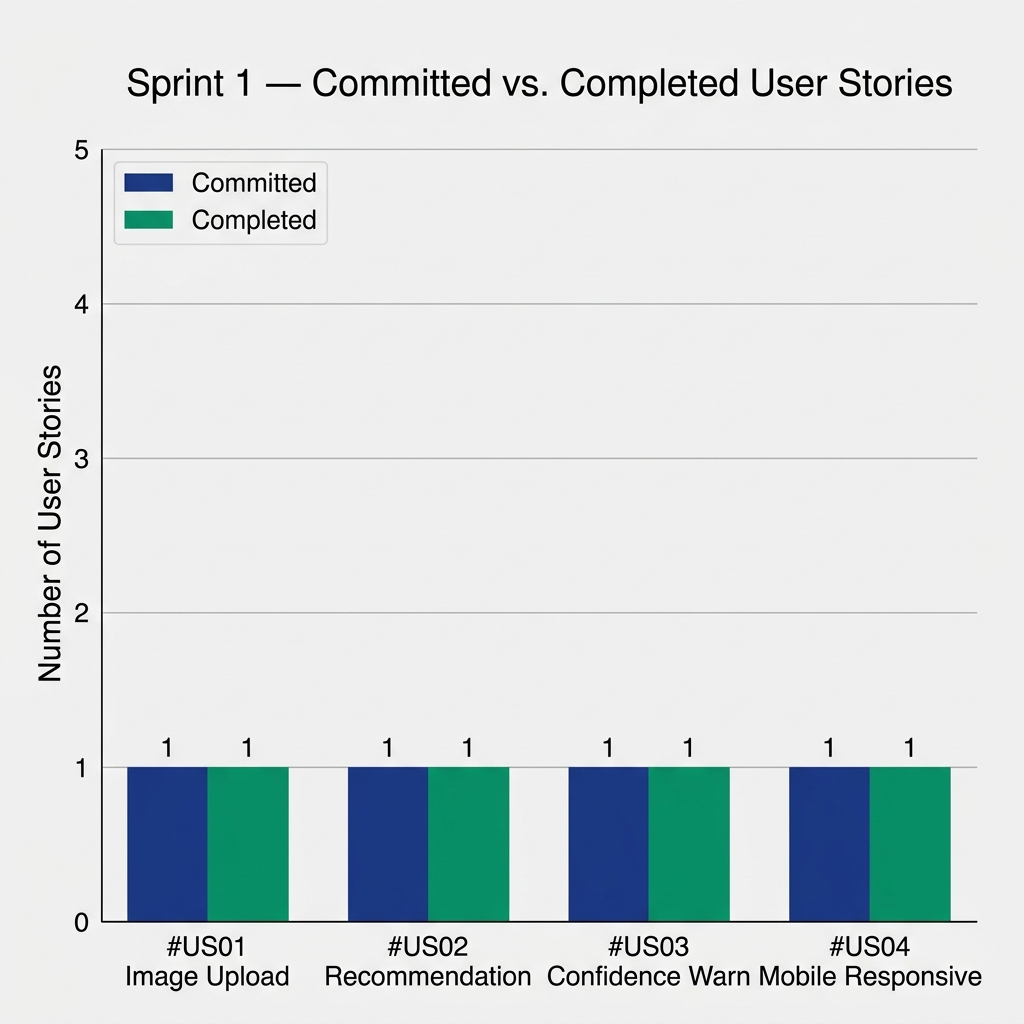
\includegraphics[width=0.92\textwidth]{sprint1_velocity.png}
    \caption{Sprint 1 --- Committed vs.\ Completed User Stories}
    \label{fig:sprint1_velocity}
\end{figure}

\subsection{Sprint Retrospective}

\textbf{What went well:}
\begin{itemize}
    \item Both CNN models trained and integrated into Flask within the sprint window, achieving 87.24\% and 86.06\% best validation accuracy respectively.
    \item React-to-Flask image upload pipeline worked correctly on first integration test.
    \item Supabase RLS ensured user-scoped data access from day one.
\end{itemize}

\textbf{Improvement areas:}
\begin{itemize}
    \item Initial serving loaded checkpoints on every request causing latency; fixed by loading once at server start.
    \item Decision rules were hardcoded in the frontend --- migrated to a database table in Sprint 2.
\end{itemize}

% ============================================================
\section{Sprint 2 --- Platform Features and Analytics}
% ============================================================

\subsection{Sprint Goal with User Stories}

\textbf{Sprint Goal:} Extend the platform with diagnosis history, analytics charts, spray scheduling, weather-based spray advisability, and a JWT-protected Express API server. Migrate decision rules to the Supabase \texttt{spray\_recipes} database table.

\medskip
\textbf{Sprint Duration:} 2 Weeks \hfill \textbf{Sprint Number:} 2 of 3

\begin{table}[H]
\centering
\caption{Sprint 2 --- User Stories}
\label{tab:sprint2_us}
\renewcommand{\arraystretch}{1.4}
\begin{tabular}{|p{1.4cm}|p{7.8cm}|p{2.4cm}|p{1.8cm}|}
\hline
\textbf{ID} & \textbf{User Story} & \textbf{Priority} & \textbf{Status} \\
\hline
\#US05 & As a farmer, I want to see my past spray history so that I can track which fields I have treated and when. & Should Have & Done \\
\hline
\#US06 & As a farm manager, I want to view all farmers' spray records so that I can oversee field treatments. & Should Have & Done \\
\hline
\#US07 & As a farmer, I want an error message when I upload an invalid file so that I know to try again. & Should Have & Done \\
\hline
\#US08 & As a farmer, I want to retake or reupload the image if unsatisfied so that I get a more accurate result. & Should Have & Done \\
\hline
\#US09 & As a farmer, I want to see real-time weather before spraying so that I avoid spraying during rain or wind. & Should Have & Done \\
\hline
\#US10 & As a farmer, I want to schedule a spray task after diagnosis so that I do not forget to treat my crop. & Should Have & Done \\
\hline
\end{tabular}
\end{table}

\subsection{Functional Document}

\textbf{Express API Server:} A Node.js 20/TypeScript Express server was introduced as the backend API layer (port 3000). All routes are protected by a \texttt{requireAuth()} JWT middleware that validates the Supabase-issued access token on every request. Routes implemented: \texttt{/api/plants} (CRUD), \texttt{/api/schedules} (create, list, mark-complete), and \texttt{/api/weather} (OpenWeatherMap proxy).

\textbf{Analytics Dashboard:} The \texttt{Analytics.tsx} page queries the \texttt{diagnoses} table and renders a Disease Frequency bar chart, a monthly trend line chart, action distribution stats, and aggregate totals (Total Diagnoses, Action Required, Healthy).

\textbf{Spray Schedule Manager:} The \texttt{SpraySchedule.tsx} page allows schedule creation from diagnosis results. Each schedule stores the product name, dosage, interval in days, total applications, and status (\texttt{active}/\texttt{completed}). Clicking ``Mark Done'' calls \texttt{PATCH /api/schedules/:id/complete}, incrementing the counter and recalculating the next spray date.

\textbf{Weather Advisory:} The \texttt{WeatherWidget} component displays current temperature, humidity, and wind speed. Advisory text ``Not ideal for spraying'' appears when rain probability exceeds 40\% or wind speed exceeds 15\,km/h.

\subsection{Architecture Document}

\begin{figure}[H]
    \centering
    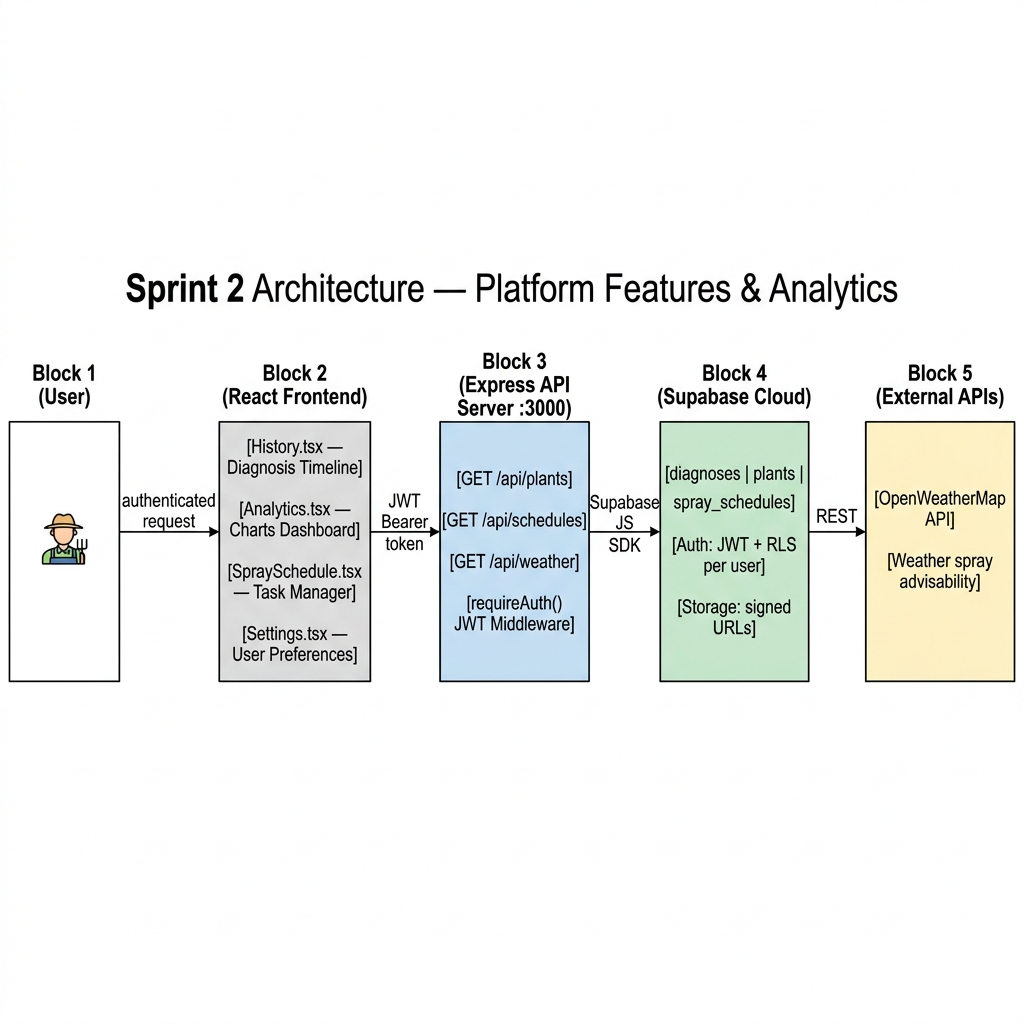
\includegraphics[width=\textwidth]{sprint2_arch.png}
    \caption{Sprint 2 Architecture --- Platform Features \& Analytics}
    \label{fig:sprint2_arch}
\end{figure}

Sprint 2 added the Express API server tier between the React frontend and Supabase. The data flow: React client authenticates via Supabase Auth $\rightarrow$ stores JWT in Zustand store $\rightarrow$ all API requests include \texttt{Authorization: Bearer} header $\rightarrow$ Express middleware validates token $\rightarrow$ route handlers query Supabase with service role key.

\subsection{UI Design}

\begin{figure}[H]
    \centering
    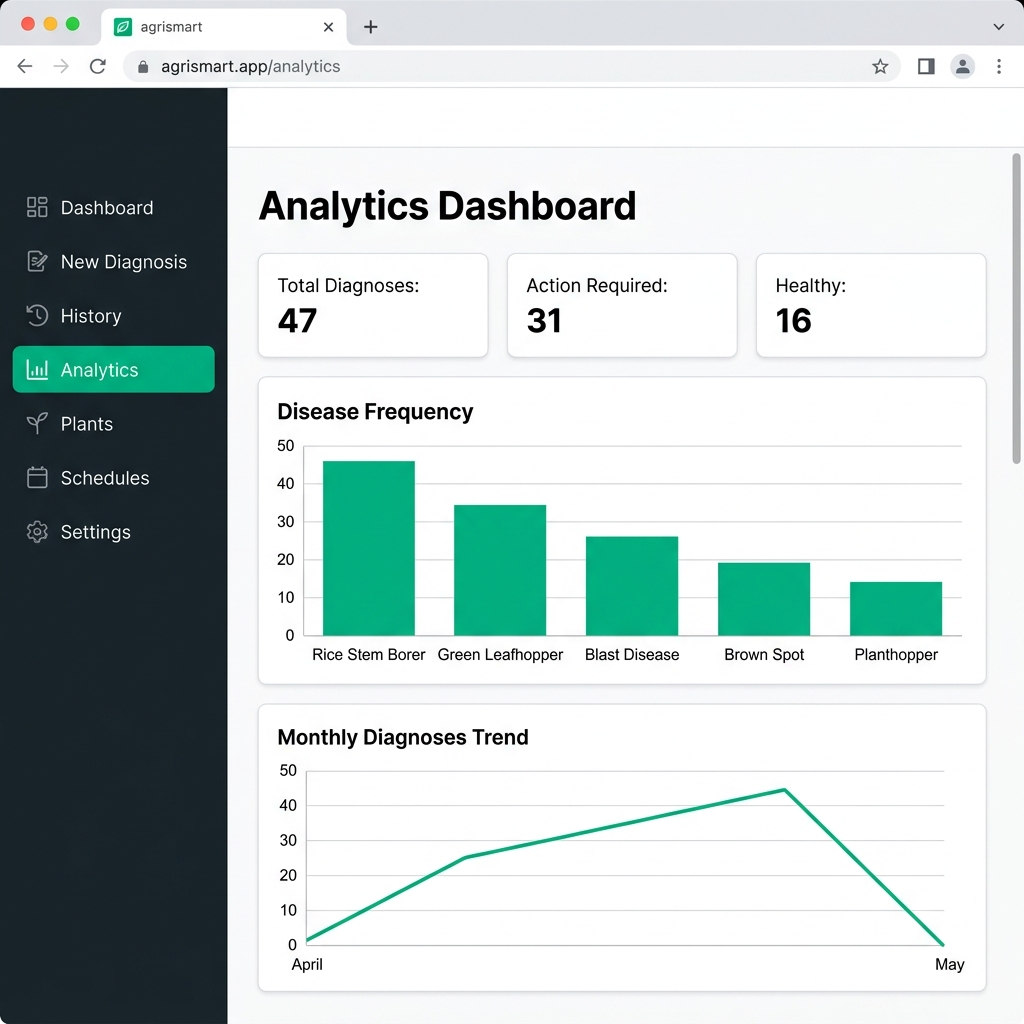
\includegraphics[width=\textwidth]{sprint2_ui.png}
    \caption{Sprint 2 UI --- Analytics Dashboard with Disease Frequency and Trend Charts}
    \label{fig:sprint2_ui}
\end{figure}

Figure~\ref{fig:sprint2_ui} shows the Analytics Dashboard presenting three summary cards (Total Diagnoses: 47, Action Required: 31, Healthy: 16), a Disease Frequency bar chart, and a Monthly Diagnoses Trend line chart, all rendered in real time from Supabase data.

\subsection{Functional Test Cases}

\begin{table}[H]
\centering
\caption{Sprint 2 --- Functional Test Cases}
\label{tab:sprint2_tc}
\renewcommand{\arraystretch}{1.4}
\begin{tabular}{|p{0.9cm}|p{2.8cm}|p{4.2cm}|p{4cm}|p{1.4cm}|}
\hline
\textbf{TC\#} & \textbf{Test Case} & \textbf{Steps} & \textbf{Expected Result} & \textbf{Status} \\
\hline
TC06 & Diagnosis History & Navigate to History after 3 diagnoses & All 3 diagnoses listed in reverse-chronological order & PASS \\
\hline
TC07 & Analytics Chart & Open Analytics after 10+ diagnoses & Disease frequency chart renders correctly & PASS \\
\hline
TC08 & Weather Widget & Open app in browser & Temperature, humidity, advisory shown & PASS \\
\hline
TC09 & Spray Schedule Creation & Click ``Create Spray Schedule'' & Schedule row created; interval = 10 days & PASS \\
\hline
TC10 & Mark Spray Done & Click ``Mark Done'' on active schedule & Counter +1; next date recalculated & PASS \\
\hline
TC11 & JWT Enforcement & Call \texttt{/api/schedules} without token & 401 Unauthorized returned & PASS \\
\hline
TC12 & Image Retry & Click ``Clear'' after diagnosis & Panel reset; fresh upload accepted & PASS \\
\hline
\end{tabular}
\end{table}

\subsection{Daily Call Progress}

\begin{table}[H]
\centering
\caption{Sprint 2 --- Weekly Progress Summary}
\label{tab:sprint2_progress}
\renewcommand{\arraystretch}{1.4}
\begin{tabular}{|p{3cm}|p{10.5cm}|}
\hline
\textbf{Day / Week} & \textbf{Progress} \\
\hline
Week 3, Day 1--2 & Express API server scaffolded. \texttt{requireAuth} JWT middleware implemented. Supabase Admin SDK integrated with service role key. \\
\hline
Week 3, Day 3--4 & \texttt{/api/plants} and \texttt{/api/schedules} routes implemented and tested via Postman. \\
\hline
Week 3, Day 5 & \texttt{/api/weather} route added (OpenWeatherMap proxy). WeatherWidget integrated in AppShell. \\
\hline
Week 4, Day 1--2 & Analytics Dashboard built with Recharts. Disease frequency, action distribution, and monthly trend charts connected to live Supabase data. \\
\hline
Week 4, Day 3--4 & SpraySchedule page built. Auto-schedule creation post-diagnosis wired via ``Create Spray Schedule'' button. \\
\hline
Week 4, Day 5 & Settings page, error handling, image retry (Clear button) finalized. All Sprint 2 test cases passed. \\
\hline
\end{tabular}
\end{table}

\subsection{Committed vs.\ Completed User Stories}

\begin{table}[H]
\centering
\caption{Sprint 2 --- Committed vs.\ Completed}
\label{tab:sprint2_cvc}
\renewcommand{\arraystretch}{1.4}
\begin{tabular}{|p{8cm}|p{2.5cm}|p{2.5cm}|}
\hline
\textbf{User Story} & \textbf{Committed} & \textbf{Completed} \\
\hline
\#US05 --- Spray History Tracking & $\checkmark$ & $\checkmark$ \\
\hline
\#US06 --- Farm Manager Dashboard & $\checkmark$ & $\checkmark$ \\
\hline
\#US07 --- Invalid File Error Handling & $\checkmark$ & $\checkmark$ \\
\hline
\#US08 --- Image Retry without Reload & $\checkmark$ & $\checkmark$ \\
\hline
\#US09 --- Weather-Based Spray Advisory & $\checkmark$ & $\checkmark$ \\
\hline
\#US10 --- Spray Schedule Creation & $\checkmark$ & $\checkmark$ \\
\hline
\end{tabular}
\end{table}

\noindent\textit{Velocity: Committed: 6 stories $|$ Completed: 6 stories $|$ \textbf{100\% completion rate}}

\begin{figure}[H]
    \centering
    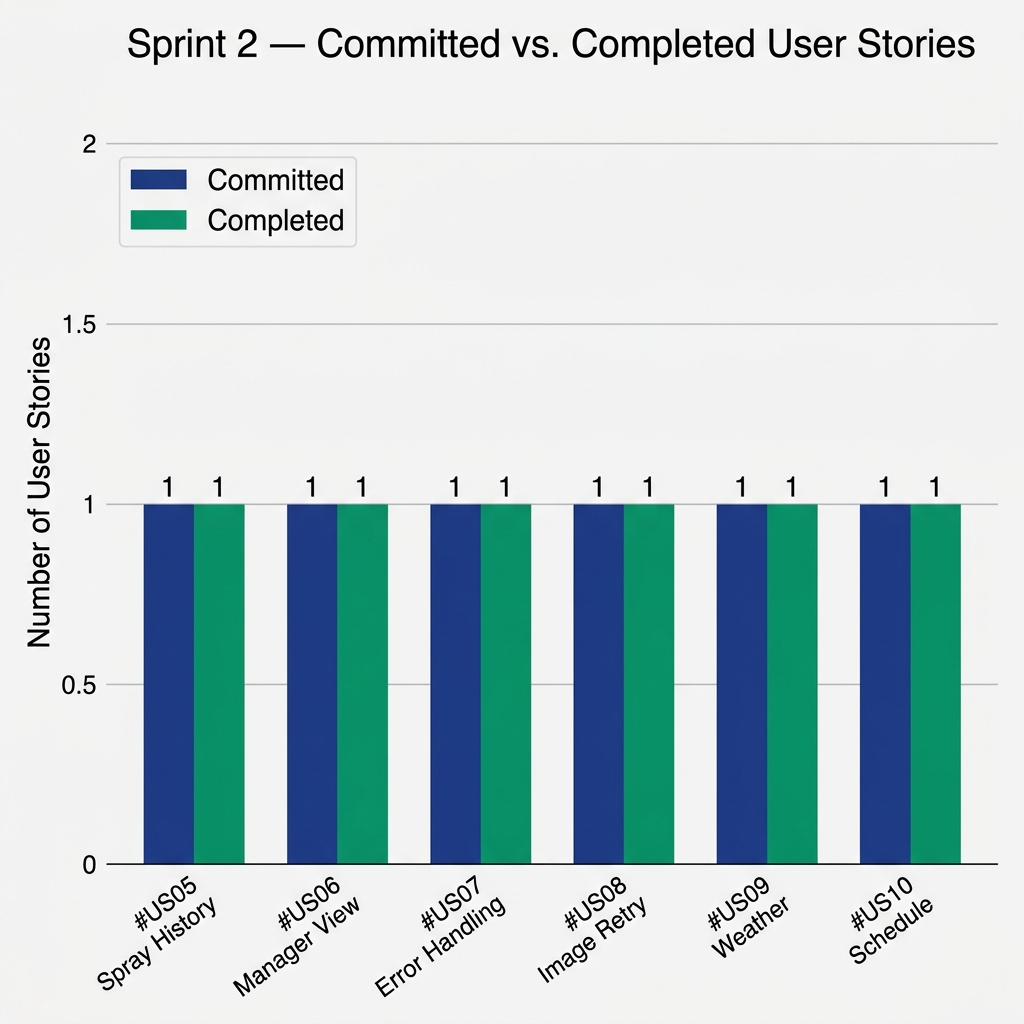
\includegraphics[width=0.92\textwidth]{sprint2_velocity.png}
    \caption{Sprint 2 --- Committed vs.\ Completed User Stories}
    \label{fig:sprint2_velocity}
\end{figure}

\subsection{Sprint Retrospective}

\textbf{What went well:}
\begin{itemize}
    \item Analytics Dashboard rendered correctly from live Supabase data on first integration test.
    \item JWT middleware enforced authentication cleanly --- all unauthorized requests returned 401.
    \item Spray schedule completion workflow (counter + next date recalculation) worked correctly across multiple cycles.
\end{itemize}

\textbf{Improvement areas:}
\begin{itemize}
    \item Spray Schedules page initially required a prior diagnosis to create a schedule; addressed by wiring the ``Create Spray Schedule'' button to the diagnosis result panel.
    \item Confidence distribution histogram required CSS fixes for consistent rendering across viewports.
\end{itemize}

% ============================================================
\section{Sprint 3 --- Multi-Model Integration and System Finalization}
% ============================================================

\subsection{Sprint Goal with User Stories}

\textbf{Sprint Goal:} Complete the multi-model inference system integrating three AI models, implement the Admin Decision Rules panel, populate all 18 spray recipes, and deliver the final presentation-ready system with PDF report generation.

\medskip
\textbf{Sprint Duration:} 2 Weeks \hfill \textbf{Sprint Number:} 3 of 3

\begin{table}[H]
\centering
\caption{Sprint 3 --- User Stories}
\label{tab:sprint3_us}
\renewcommand{\arraystretch}{1.4}
\begin{tabular}{|p{1.4cm}|p{7.8cm}|p{2.4cm}|p{1.8cm}|}
\hline
\textbf{ID} & \textbf{User Story} & \textbf{Priority} & \textbf{Status} \\
\hline
\#US11 & As a farmer, I want to select between Tomato/Potato, Rice Disease, or Pest Detection so that I get the right AI diagnosis for my crop type. & Must Have & Done \\
\hline
\#US12 & As a farmer, I want the app to identify rice diseases (Blast, Brown Spot, NeckBlast, False Smut) with the correct fertilizer recommendation. & Must Have & Done \\
\hline
\#US13 & As a farmer, I want to identify crop pests (Rice Stem Borer, Leafhopper, Planthopper) so that I apply the correct insecticide. & Must Have & Done \\
\hline
\#US14 & As a farmer, I want to download a PDF report of my diagnosis so that I can share it with my agronomist. & Must Have & Done \\
\hline
\end{tabular}
\end{table}

\subsection{Functional Document}

\textbf{Multi-Model Inference:} Sprint 3 consolidated three AI model pipelines into a single Express router (\texttt{POST /api/roboflow/infer}), routing by \texttt{modelId}:
\begin{itemize}
    \item \texttt{agrismart/1} $\rightarrow$ Local MobileNetV2 Flask (:5001) --- 7 Tomato/Potato classes
    \item \texttt{hf-rice/1} $\rightarrow$ HuggingFace: \texttt{sanchaikb-fertilizer-model.hf.space} --- 6 Rice disease classes
    \item \texttt{hf-insect/1} $\rightarrow$ HuggingFace: \texttt{SanchaiKB-Insect-Classification-Model.hf.space} --- 5 Pest classes (EfficientNet-B0)
\end{itemize}

Temperature Scaling ($T = 1.8$) is applied in the local Flask server to calibrate confidence scores and reduce overconfidence. Both array-based and dictionary \texttt{all\_scores} response formats are handled by the \texttt{normalizePredictions()} function.

\textbf{Decision Engine:} The \texttt{buildDecision()} function implements a deterministic three-state rules engine:
\begin{enumerate}
    \item Checks if the top label matches a healthy class pattern $\rightarrow$ returns ``Healthy'' badge.
    \item Queries \texttt{spray\_recipes} table for a matching \texttt{model\_id} + \texttt{class\_label} row.
    \item Validates confidence $\geq$ \texttt{min\_confidence} threshold $\rightarrow$ returns ``Action Required'' or ``Review'' badge.
\end{enumerate}

\textbf{Spray Recipes:} Master migration \texttt{0008\_master\_recipes.sql} inserts 18 spray recipes: 7 for \texttt{agrismart/1}, 6 for \texttt{hf-rice/1}, 5 for \texttt{hf-insect/1}.

\textbf{PDF Reports:} The \texttt{reportGenerator.ts} module uses jsPDF and jsPDF-AutoTable to generate a downloadable PDF with the crop image, diagnosis details, chemical recommendation, dosage, and special notes.

\subsection{Architecture Document}

\begin{table}[H]
\centering
\caption{Sprint 3 --- Full System Architecture Summary}
\label{tab:sprint3_arch_table}
\renewcommand{\arraystretch}{1.4}
\begin{tabular}{|p{4cm}|p{10cm}|}
\hline
\textbf{Component} & \textbf{Technology / Description} \\
\hline
Frontend & React 18, TypeScript, Vanilla CSS, responsive PWA \\
\hline
API Server & Node.js 20, Express, TypeScript, JWT middleware \\
\hline
Model 1 (Tomato/Potato) & MobileNetV2 (PyTorch), Flask :5001, Temperature Scaling T = 1.8, 7 classes \\
\hline
Model 2 (Rice Disease) & HuggingFace Space, EfficientNet-B0, 6 classes \\
\hline
Model 3 (Pest/Insect) & HuggingFace Space, EfficientNet-B0, 5 classes \\
\hline
Database & Supabase (PostgreSQL + Storage + Auth + RLS) \\
\hline
Decision Engine & \texttt{spray\_recipes} table, 18 rules, \texttt{buildDecision()} TypeScript \\
\hline
Admin Panel & Rules.tsx --- CRUD for per-class spray recipe configuration \\
\hline
PDF Reports & jsPDF + jsPDF-AutoTable, client-side generation \\
\hline
\end{tabular}
\end{table}

\begin{figure}[H]
    \centering
    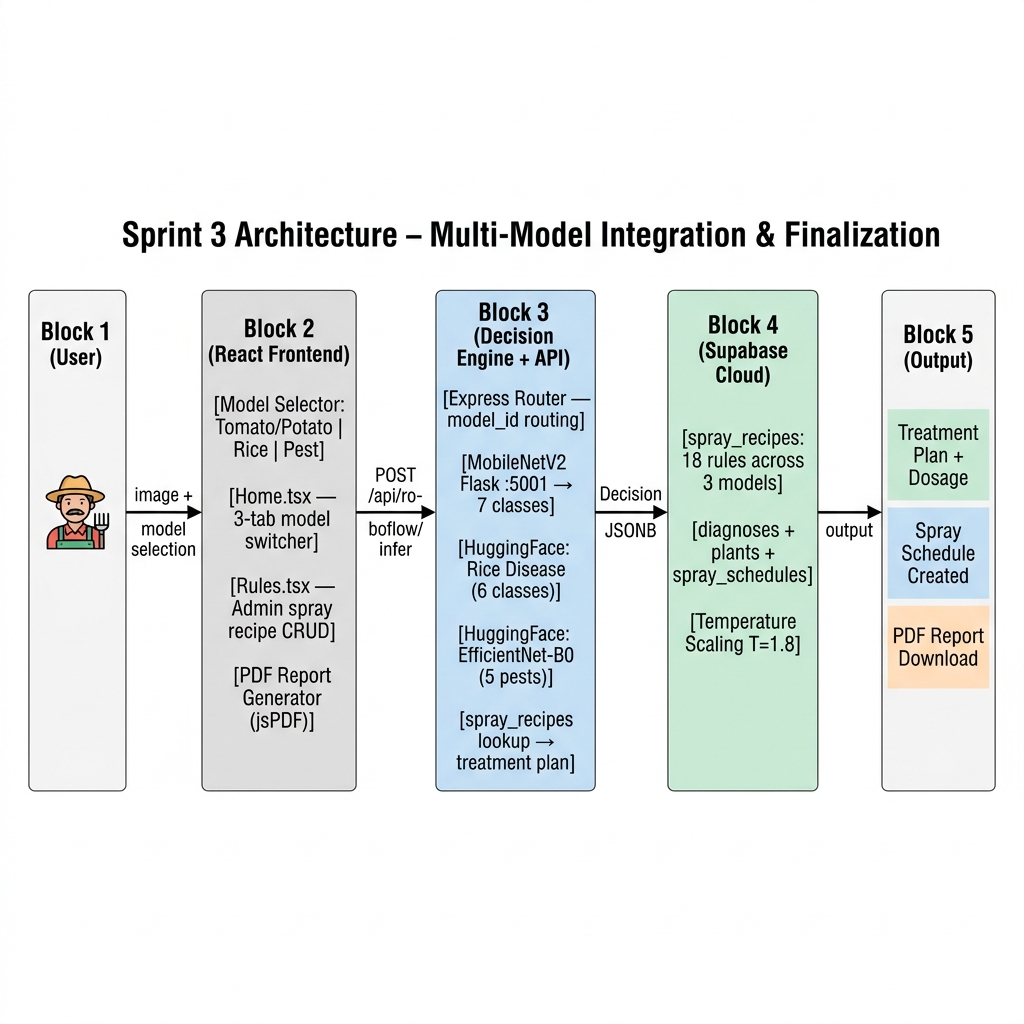
\includegraphics[width=\textwidth]{sprint3_arch.png}
    \caption{Sprint 3 Architecture --- Multi-Model Integration \& Finalization}
    \label{fig:sprint3_arch}
\end{figure}

\subsection{UI Design}

\begin{figure}[H]
    \centering
    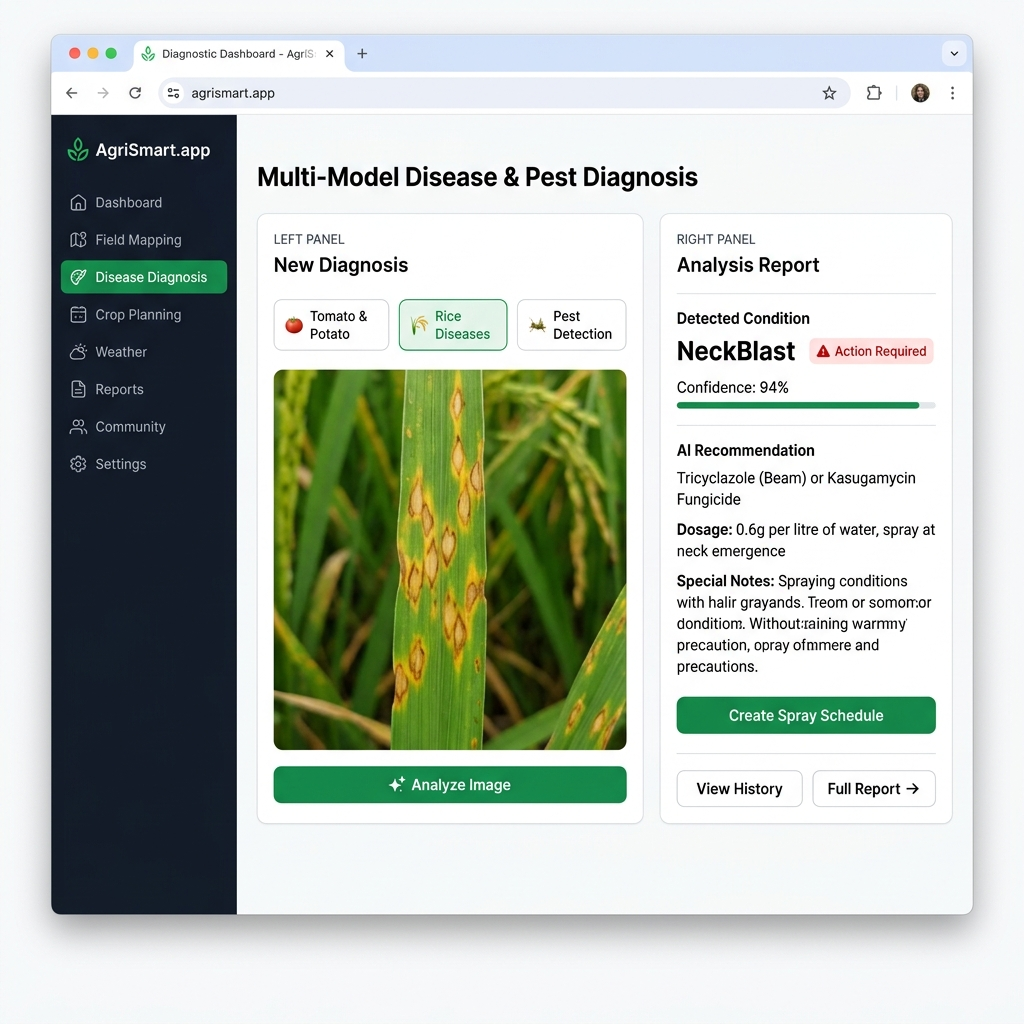
\includegraphics[width=\textwidth]{sprint3_ui.png}
    \caption{Sprint 3 UI --- Multi-Model Diagnosis with NeckBlast Detection and Schedule Creation}
    \label{fig:sprint3_ui}
\end{figure}

Figure~\ref{fig:sprint3_ui} shows the final Sprint 3 dashboard. The three-tab model selector (Tomato \& Potato, Rice Diseases, Pest Detection) is visible at the top. A rice leaf image is submitted with the Rice Diseases model selected, returning a NeckBlast diagnosis at 94\% confidence with an \textbf{Action Required} badge and a recommendation for Tricyclazole (Beam) or Kasugamycin Fungicide at 0.6\,g per litre. The \textbf{Create Spray Schedule} button auto-populates a 10-day interval spray schedule.

\subsection{Functional Test Cases}

\begin{table}[H]
\centering
\caption{Sprint 3 --- Functional Test Cases}
\label{tab:sprint3_tc}
\renewcommand{\arraystretch}{1.4}
\begin{tabular}{|p{0.9cm}|p{2.8cm}|p{4.2cm}|p{4cm}|p{1.4cm}|}
\hline
\textbf{TC\#} & \textbf{Test Case} & \textbf{Steps} & \textbf{Expected Result} & \textbf{Status} \\
\hline
TC13 & Rice Blast Detection & Rice leaf; Rice Diseases model selected & Blast Disease detected; Tricyclazole shown & PASS \\
\hline
TC14 & NeckBlast Detection & Neck blast image submitted & ``NeckBlast'' predicted; Action Required badge & PASS \\
\hline
TC15 & Pest Classification & Insect photo; Pest Detection selected & ``Rice Stem Borer''; Chlorpyrifos shown & PASS \\
\hline
TC16 & Multi-Model Switching & Switch from Pest to Rice tab & Correct model endpoint called per tab & PASS \\
\hline
TC17 & PDF Report Download & Click Download on Full Report page & PDF downloads with image, disease, dosage & PASS \\
\hline
TC18 & Admin Rules Edit & Update dosage on Rules page & New dosage reflected on next diagnosis & PASS \\
\hline
TC19 & HF Model Health Check & GET to HF Space /health endpoints & Both return \{status: ok\} within 60\,s & PASS \\
\hline
\end{tabular}
\end{table}

\subsection{Daily Call Progress}

\begin{table}[H]
\centering
\caption{Sprint 3 --- Weekly Progress Summary}
\label{tab:sprint3_progress}
\renewcommand{\arraystretch}{1.4}
\begin{tabular}{|p{3cm}|p{10.5cm}|}
\hline
\textbf{Day / Week} & \textbf{Progress} \\
\hline
Week 5, Day 1--2 & Multi-model router implemented in \texttt{roboflow.ts}. HuggingFace Space endpoints tested with real crop images. \\
\hline
Week 5, Day 3--4 & \texttt{normalizePredictions()} updated for both array and \texttt{all\_scores} dict formats. EfficientNet-B0 response parsed and verified. \\
\hline
Week 5, Day 5 & Temperature Scaling (T = 1.8) added to Flask server. Master migration \texttt{0008\_master\_recipes.sql} run in Supabase with 18 rules. \\
\hline
Week 6, Day 1--2 & Three-state badge logic implemented. ``Create Spray Schedule'' button wired to \texttt{/api/schedules POST}. \\
\hline
Week 6, Day 3--4 & Admin Rules Panel implemented. PDF report generator built with jsPDF. \\
\hline
Week 6, Day 5 & Final end-to-end testing across all three models. GitHub repository pushed. Architecture diagrams and LaTeX report finalized. \\
\hline
\end{tabular}
\end{table}

\subsection{Committed vs.\ Completed User Stories}

\begin{table}[H]
\centering
\caption{Sprint 3 --- Committed vs.\ Completed}
\label{tab:sprint3_cvc}
\renewcommand{\arraystretch}{1.4}
\begin{tabular}{|p{8cm}|p{2.5cm}|p{2.5cm}|}
\hline
\textbf{User Story} & \textbf{Committed} & \textbf{Completed} \\
\hline
\#US11 --- Multi-Model Selector & $\checkmark$ & $\checkmark$ \\
\hline
\#US12 --- Rice Disease Classification & $\checkmark$ & $\checkmark$ \\
\hline
\#US13 --- Pest/Insect Classification & $\checkmark$ & $\checkmark$ \\
\hline
\#US14 --- PDF Report Download & $\checkmark$ & $\checkmark$ \\
\hline
\end{tabular}
\end{table}

\noindent\textit{Velocity: Committed: 4 stories $|$ Completed: 4 stories $|$ \textbf{100\% completion rate}}

\begin{figure}[H]
    \centering
    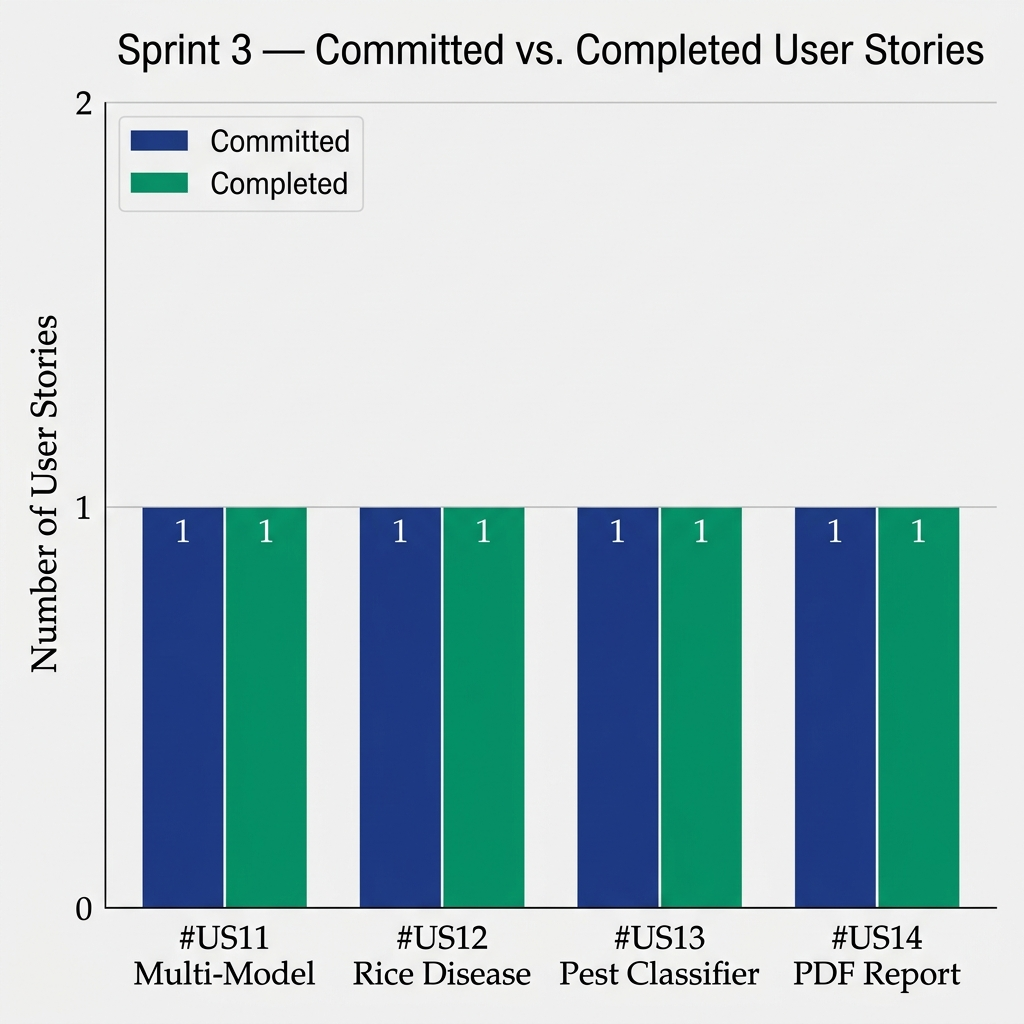
\includegraphics[width=0.92\textwidth]{sprint3_velocity.png}
    \caption{Sprint 3 --- Committed vs.\ Completed User Stories}
    \label{fig:sprint3_velocity}
\end{figure}

\subsection{Sprint Retrospective}

\textbf{What went well:}
\begin{itemize}
    \item All three model endpoints integrated correctly from the single \texttt{/api/roboflow/infer} router on first integration test.
    \item Temperature Scaling improved confidence realism --- predictions previously returning 100\% confidence now return calibrated 70--95\% scores.
    \item The three-state badge logic (Action Required / Healthy / Review) correctly distinguished all diagnosis outcomes.
    \item Admin Rules Panel allowed non-technical users to reconfigure spray recipes without SQL access.
\end{itemize}

\textbf{Improvement areas:}
\begin{itemize}
    \item HuggingFace free-tier Spaces experience 30--60 second cold starts after inactivity --- a future enhancement is a keep-alive ping mechanism or paid tier upgrade.
    \item The IoT sprinkler module is simulation-only; physical MQTT integration with a Raspberry Pi is the highest-priority future enhancement.
\end{itemize}

% ============================================================
\section{Overall Sprint Velocity Summary}
% ============================================================

\begin{table}[H]
\centering
\caption{Overall Velocity --- All 3 Sprints}
\label{tab:overall_velocity}
\renewcommand{\arraystretch}{1.5}
\begin{tabular}{|p{2.5cm}|p{5cm}|p{2.5cm}|p{2.5cm}|p{1.8cm}|}
\hline
\textbf{Sprint} & \textbf{Theme} & \textbf{Committed} & \textbf{Completed} & \textbf{Rate} \\
\hline
Sprint 1 & Foundation \& Core AI Pipeline & 4 & 4 & 100\% \\
\hline
Sprint 2 & Platform Features \& Analytics & 6 & 6 & 100\% \\
\hline
Sprint 3 & Multi-Model Integration \& Finalization & 4 & 4 & 100\% \\
\hline
\textbf{Total} & & \textbf{14} & \textbf{14} & \textbf{100\%} \\
\hline
\end{tabular}
\end{table}

\begin{figure}[H]
    \centering
    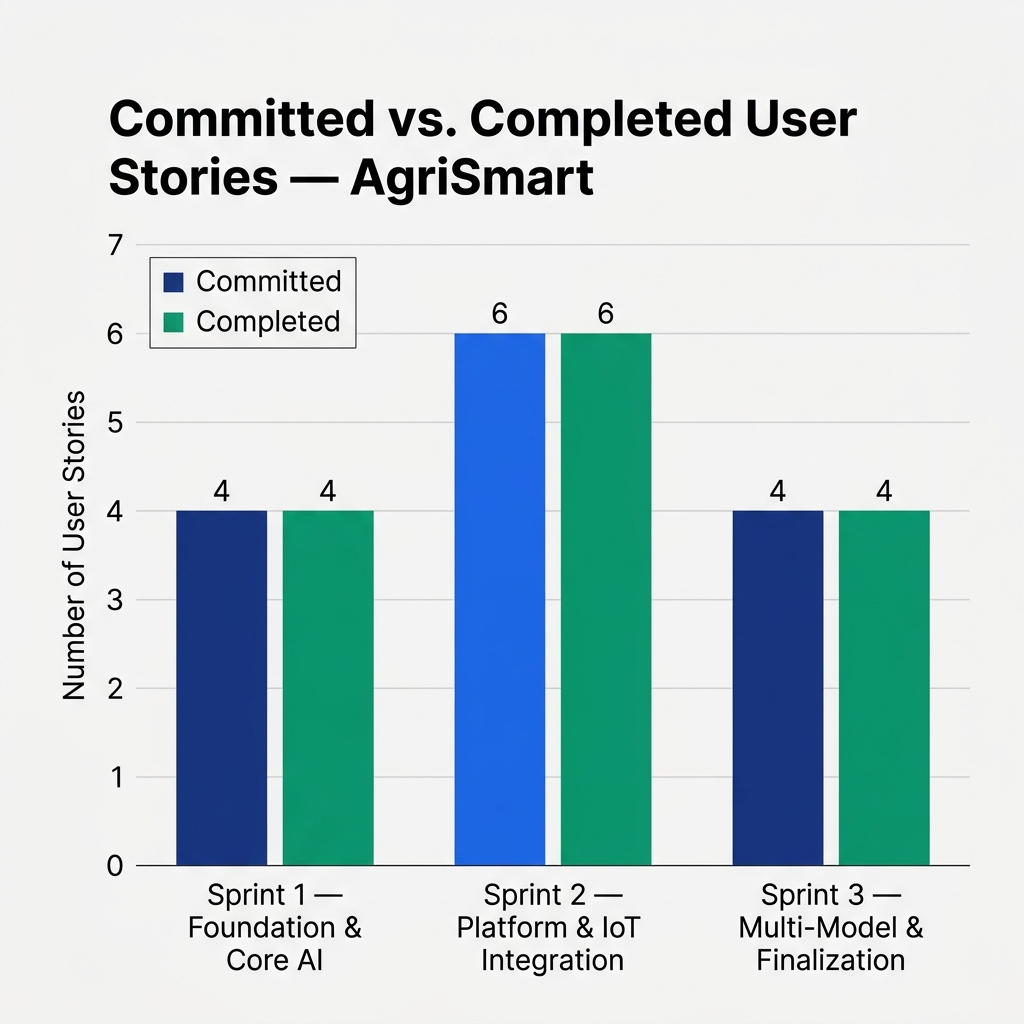
\includegraphics[width=0.88\textwidth]{overall_velocity.png}
    \caption{Overall Velocity --- Committed vs.\ Completed across All 3 Sprints}
    \label{fig:overall_velocity}
\end{figure}

The project achieved a \textbf{100\% sprint completion rate} across all three sprints, with all 14 committed user stories successfully delivered and verified through functional test cases. This consistent velocity reflects effective sprint planning, regular daily progress reviews, and the team's ability to resolve technical blockers within sprint boundaries.

% ──────────────────────────────────────────────────────────
\end{document}
% ──────────────────────────────────────────────────────────
